\begin{introduction}
    \item 体系中态的描述
    \item 算符的基本性质
    \item 态空间物理量的表征
    \item 状态的演化
    \item $|r\rangle$和$|p\rangle$表象
    \item 概率幅与测量拾遗
    \item *态空间的张量积基础
    \item *密度矩阵简介
\end{introduction}

在第一章中我们已经知道了任何一个物理理论都应该面对以下三个基本问题:
\begin{itemize}
    \item 系统的状态如何描述?
    \item 如何通过系统的状态求得各种宏观物理量?
    \item 状态的演化规律是什么??
\end{itemize}

下面我们基于量子力学的实验事实,通过提出量子力学的若干基本假设以回答这三个问题:
\section{体系中态的描述}
    \subsection{波函数}
    与经典物理不同的地方在于,此时提出的理论需要基于粒子的波粒二象性。我们先从经典物理中寻找灵感:无论是机械波,还是电磁学中的电场强度和磁场强度,我们都能构建波动函数形式$u(r,t)$,而这个物理量能够描述粒子的全部信息。相对应的,我们引入一个类似的波动函数——波函数$\psi(r,t)$,同时进一步假设波函数能够描述基于波粒二象性粒子的全部信息。于是有以下假设:
    \begin{definition}{波函数公设Ⅰ}{wavefunc1}
    在波粒二象性的框架下,我们用一个时空函数波函数$\Psi(r,t) $描述粒子的全部信息。
    \end{definition}
    
    但是,遗憾的是,我们无法说明物质波是某个正是可测物理量的波动,因此波函数是一个不客观测量,换句话说波函数本身本身是没有物理意义的。在1926年,Born给出了波函数的统计诠释。那么什么是统计诠释呢?在这里我们举一个例子:考虑平面波$A\exp{i\Vec{k}\cdot\Vec{r}-i\omega t}$,由于波幅的平方与波的强度$I$成正比,同时波的强度又与波的数密度大小成正比,即:
    \begin{equation}
        n\sim I\sim A^2
    \end{equation}
    
    进一步,如果从概率的角度来考虑,数密度越大,则在该区域附近的概率密度越大。由于电子衍射实验与光的衍射实验结果十分相似,因此我们可以将平面波的性质迁移到波函数的理解上。于是我们自然假设波函数模的平方表示粒子在该区域附近的概率密度。这个假设同时自然说明波函数是基于统计思想的。
    \begin{definition}{波函数公设Ⅱ}{wavefunc2}
        波函数模的平方表示粒子在该区域附近出现的概率密度。
    \end{definition}
 
 此外,在非相对论条件下,粒子不会产生和湮灭,那么粒子在全空间出现的概率之和应该为1:
 \begin{equation}
      \int_{\Omega}|\Psi(r,t)|^2dr=1
 \end{equation}

这个性质被称为归一性。这促使我们去思考波函数所在的空间应该是平方可积函数\footnote{平方可积的定义如下:
\begin{equation*}
    \int_{\Omega} |f(r)|^2dr<\infty
\end{equation*}
}的集合,在数学上我们称之为Hilbert空间($L^2$空间)。但是波函数所在空间并不只有平方可积一个限制条件。波函数的统计诠释限制了波函数并不是可以随意取定的,它需要满足连续、单值、有限三个性质。其中连续是波形式的表现,因为对于一种波,我们当然不允许出现不连续的奇异点\footnote{进一步,我们往往也会要求波函数的1阶导也是连续的}出现;单值是统计诠释的体现,即一个地方只能有一个概率;有限是保证概率是有意义的。因此,波函数空间$\mathscr{F}$实际上是Hilbert空间的子空间。

最后想讨论一下波函数在物理层面的等价性。因为概率本身是相对的,你去谈孤立位置上的概率是没有意义的,我们在意的性质是空间上的概率分布,这种由概率导致的相对性导致$C\Psi(r,t)$和$\Psi(r,t)$的概率分布是一样的。于是这两个波函数所描述的对应粒子的运动规律也完全一样,在量子力学中我们就不区分这两个波函数的区别了。同样,$\Psi(r,t)$与乘上相位因子的波函数$\Psi(r,t)e^{i\alpha t}$相比,由于两者模的平方相等,因此在量子力学描述整体运动规律的时候往往不考虑相位的作用\footnote{但是相位对于测量性质有较大影响。}。
    \subsection{波函数空间$\mathscr{F}$上的基}
    本节我们讨论一下波函数空间$\mathscr{F}$的性质。首先,根据上节的性质,我们已经了解了$\mathscr{F}$是$L^2$空间的子空间,因此其一定是一个复内积空间空间,由此我们可以简单的定义空间上的内积与范数:
    \begin{align}
        \begin{split}
            (\varphi,\psi)=&\int_{-\infty}^{+\infty}\varphi^{*}(r)\psi(r)d^3r\\
            |\psi(r)|=&\sqrt{(\psi,\psi)}
        \end{split}
    \end{align}
    
    通过线性代数的学习,我们知道要研究一个线性空间,最直接的办法就是选取空间上的一组基,这样我们就可以用基对应的坐标表示空间中的任意一个矢量\footnote{这里的本质在于:如果确定一组基,那么线性空间与其对应的坐标空间是同构的。}。但是与线性代数不同的地方在于,我们可以选取$\mathscr{F}$上的一组“连续基”。为了更好的理解相关概念,我们先从熟悉的离散情况讨论:
    
    首先讨论$\mathscr{F}$上离散的正交归一基$\{u_i\}$,我们知道对于内积空间上的正交归一基,空间中任意一个矢量$\psi$可以写成:
    \begin{equation}
        \psi=\sum_{i}c_iu_i
    \end{equation}
    
    由于$\{u_i\}$满足正交归一性:
    \begin{equation}
        (u_i,u_j)=\delta_{ij}
    \end{equation}
    
    因此展开系数$c_i$是$\psi$到$u_i$的投影:
    \begin{equation}
        c_i=(u_i,\psi)=\int u_i^{*}(r)u_i(r)d^3r
    \end{equation}
   
    
    上三式联立即可得\footnote{这里我们默认了上述函数都可以交换求和号和积分号,但是这里需要严谨的数学证明。}:
    \begin{align}
        \begin{split}
            \psi=&\sum_i\Big(\int u_i^{*}(r')u_i(r')d^3r'\Big)u_i(r)\\
            =&\int \Big(\sum_i u_i^*(r)u_i(r) \Big)\psi(r')d^3r'
        \end{split}
    \end{align}
    
    如果上式恒成立,则一定有关系:
    \begin{equation}
        \sum_i u_i^*(r)u_i(r)=\delta(r-r')
    \end{equation}
    
    由于上式成立的前提是$\{u_i\}$是$\mathscr{F}$上的一组正交归一基,因此我们可以将上式看作函数组$\{u_i\}$具有封闭性的依据。
    
    正交归一基的优势之一在于极大的简化了标量积的计算:假设$\mathscr{F}$上有两个波函数$\varphi,\psi$,它们一定能够被$\{u_i\}$线性表示:
    \begin{align}
        \begin{split}
            \varphi=&\sum_i b_i u_i\\
            \psi =& \sum_i c_i u_i
        \end{split}
    \end{align}
    
    那么两个波函数的标量积可以表示为:
    \begin{equation}
        (\varphi,\psi)=\Big(\sum_i b_i u_i,\sum_j b_j u_j\Big)= \sum_{i,j}b_i^*c_j(u_i,u_j)=\sum_{i,j}b_i^*c_j\delta_{ij}=\sum_{i,j}b_i^*c_j
    \end{equation}
    
    类似的,我们可以将结论拓展到“连续基”上。何谓连续基呢?我们定义:以$\alpha$为连续指标的函数$\{\omega_{\alpha}(r)\}$为$\mathscr{F}$上的连续基。与离散基$\{u_i\}$对应,我们需要$\{\omega_{\alpha}(r)\}$也满足“正交归一性”以及封闭性\footnote{这里注意正交归一性打了引号的原因是:当$\alpha=\alpha'\textrm{时},(\omega_{\alpha},\omega_{\alpha})=\infty$,这表明我们在这里定义的连续基不是$\mathscr{F}$上的基。但是在实际使用中,我们发现了选取这样的连续基对计算的便利性,如$\xi_{r_0}(r)=\delta(r-r_0),v_{p_0}(p)=(2\pi\hbar)^{-\frac{3}{2}}\exp(\frac{i}{\hbar}p_0\cdot r)$。因此我们在这里仍然使用,但是我们需要铭记$\omega_{\alpha}$实际上并不具有实际物理意义。}:
    \begin{align}
        \begin{split}
            (\omega_{\alpha},\omega_{\alpha'})=\int d^3r \omega_{\alpha}(r)\omega_{\alpha'}(r)=\delta(\alpha-\alpha')\\
            \int d\alpha \omega_\alpha^*(r')\omega_\alpha(r)=\delta (r-r') 
        \end{split}
    \end{align}
    
    有了上面的定义,我们可以将$\mathscr{F}$中的任意波函数用$\{\omega_\alpha\}$展开:
    \begin{equation}
        \psi(r)=\int d\alpha c(\alpha)\omega_\alpha(r)
    \end{equation}
    
    其中展开系数$c(\alpha)$同样可以写成波函数向连续基投影的形式:
    \begin{equation}
        c(\alpha)=\int d^3r' \omega_\alpha(r')\psi(r')
    \end{equation}
    
    同样的,我们还可以建立$\omega_{\alpha'}$上两个波函数的标量积:
    \begin{align}
        \begin{split}
            (\varphi,\psi)=&\Big(\int d\alpha'b(\alpha')\omega_{\alpha'}(r)\Big)^*\int d\alpha c(\alpha)\omega_{\alpha}(r)\\
            =&\int b^*(\alpha')c(\alpha)d\alpha' \int\omega_{\alpha'}^*(r)\omega_{\alpha}(r)d\alpha\\
            =&\int b^*(\alpha')c(\alpha)d\alpha'\delta(\alpha-\alpha')\\
            =& \int d\alpha b^*(\alpha)c(\alpha)
        \end{split}
    \end{align}
        
 \subsection{态空间$\mathscr{E}$与Dirac符号}\label{subsection:Diracnotation}
 在之前的章节中,我们知道了波函数描述系统的状态,而波函数可以用波函数空间$\mathscr{F}$中的一组基(离散基或连续基)进行展开。在线性代数中,我们知道只要选定一组基,那么我们就可以用展开系数(或者可以称之为该基下的坐标)来描述空间中任意一个点。于是,当我们在波函数空间$\mathscr{F}$上选取离散基$\{u_i\}$和连续基$\{\omega_\alpha(r)\}$时,我们可以用展开系数$c_i,c(\alpha)$来描述波函数$\psi(r)$,甚至波函数$\psi(r)$在$r=r_0$处的取值也可以看作$\psi(r)$在基$\xi_{r_0}(r)$下的坐标。那么如何才能更简单的描述它们呢?
 
 此时我们类比一般的几何空间$\mathbb{R}^3$,我们可以取诸如直角坐标、极坐标、柱坐标等不同的坐标形式表达空间中的点,但是无论用哪种坐标描述,矢量的概念和运算并不随坐标的具体运算而发生改变。由此在波函数所在空间内,我们类似的引出态矢量的概念。此时我们定义粒子的每种量子态分别对应一个态矢量,记作$|\psi\rangle$(我们常称为右矢)。态矢量的集合是一个抽象空间,容易验证它也是Hilbert空间的子空间,我们称其为粒子的态空间,用$\mathscr{E}$表示。
 
 由于$\mathscr{E}$是一个复内积空间,因此我们需要讨论一下其上标量积的结构。如果我们将标量积的导出看成$\mathscr{E}\rightarrow\mathbb{F}$上的线性泛函$\chi$的话,那么根据线性代数的知识,我们知道所有线性泛函的集合同样构成一个线性空间,我们称为态空间的对偶空间,记作$\mathscr{E}^*$。同时我们将$\mathscr{E}^*$中的元素称为左矢,记作$\langle\chi|$。于是我们可以如此书写标量积:
 \begin{equation}
     \chi(|\psi\rangle)=\langle\chi|\psi\rangle
 \end{equation}
 
 下面就左矢和右矢的对应关系做一些讨论。由于态空间中的右矢一定存在模方(因为要定义概率密度),而模方的概念是由标量积定义的,因此态空间中的每一个点一定存在标量积。换句话说,一定存在一个双线性函数$\chi$,使得:
 \begin{equation}
     \chi(|\psi\rangle)=\langle\chi|\psi\rangle
 \end{equation}
 
 但是左矢不一定对应一个右矢,因为在上一节中我们已经导论过,波函数中的连续基$\omega_\alpha\notin\mathscr{F}$,因此在态空间$\mathscr{E}$中自然找不到与$\omega_\alpha$相对应的右矢;但是由于连续基与$\mathscr{E}$中的态矢量构成的标量积是存在的(比如展开系数$\langle u_i|\psi\rangle$),因此我们可以在$\mathscr{E}$中找到对应的左矢。上述内容说明左矢和右矢不是对称的,换而言之$\mathscr{E}^*$是要比$\mathscr{E}$要“大”的。为了计算与使用的方便,我们需要将这些连续基对应的函数扩充进$\mathscr{E}$中,称为广义右矢\footnote{这也就表明我们平时所用的态空间$\mathscr{E}$并不是所有的态都是具有实际物理意义的},这样就解决了左矢与右矢的不对称性。
 
 于是我们就可以构造出广义右矢\footnote{后面无特殊说明,一律简称右矢}与左矢的对应关系表达式。根据内积的定义\footnote{这里为了凸显右矢与左矢的对应关系,因此采用了一般的内积符号,后文如果没有说明的话全部采用Dirac符号}:
 \begin{equation}
     (\lambda_1|\varphi\rangle+\lambda_2|\varphi\rangle,|\psi\rangle)=\lambda_1^*\langle\varphi_1|\psi\rangle+\lambda_2^*\langle\varphi|\psi\rangle=(\lambda_1^*\langle\varphi_1|+\lambda_2^*\langle\varphi_2|,|\psi\rangle)
 \end{equation}
 
 因此右矢与左矢的关系为:
 \begin{equation}
     \lambda_1|\varphi_1\rangle+\lambda_2|\varphi_2\rangle\Longleftrightarrow \lambda_1^*\langle\varphi_1|+\lambda_2^*\langle\varphi_2|
 \end{equation}
 
 上式的对应关系也被称为反线性关系。
\section{态空间$\mathscr{E}$中算符的一般性质}
    \subsection{算符的基本性质}
        讨论了态空间以后,我们为了建立态空间上态矢量之间的变换关系(即映射),我们引入了算符的概念。如果算符$\hat{A}$将态矢量$|\psi\rangle$变为$|\psi'\rangle$,则有:
        \begin{equation}
            |\psi'\rangle =\hat{A}|\psi\rangle
        \end{equation}
        
        由此我们可以引入量子力学第二个假设:
        \begin{definition}{算符公设}{operator}
            每一个可以测量的物理量A都可以被态空间$\mathscr{E}$上起作用的一个线性算符$\hat{A}$描述,$\hat{A}$是一个测量算符。
        \end{definition}
        
        根据已经知道的两个假设来看,我们可以发现,量子力学与经典力学不同的地方在于:经典力学可以用物理量直接描述体系的状态;而量子力学是用矢量描述态,用算符描述物理量\footnote{将算符与物理量相联系看似有些无厘头,读者可以先阅读下一节的内容以获得一定的物理图像。}。
        
        在量子力学体系中,最常见的算符自然就是线性算符了。在附录中,我们提到了线性算符作用的几何直观是不改变零点的位置,同时不扭曲空间,这个物理图像能够解释相关实验的现象。简单说来,线性算符需要满足两条性质(即保持加法与数乘运算):
        \begin{align}
            \begin{split}
                 \hat{A}(|\psi_1\rangle+|\psi_2\rangle)=&\hat{A}|\psi_1\rangle+\hat{A}|\psi_2\rangle\\
                \hat{A}(|\psi\rangle a)=&(\hat{A}|\psi\rangle)a
            \end{split}
        \end{align}
        
        但是不是所有的算符都是线性的,在后文有关对称性的讨论中,我们会提及时间反演算符是一个反线性算符。反线性算符同样需要满足两条性质:
        \begin{align}
            \begin{split}
                    \hat{A}(|\psi_1\rangle+|\psi_2\rangle)=&\hat{A}|\psi_1\rangle+\hat{A}|\psi_2\rangle\\
                \hat{A}(|\psi\rangle a)=&(\hat{A}|\psi\rangle)a^*
            \end{split}
        \end{align}
        
        我们可以发现反线性算符与线性算符不同的地方就在于数乘的映射,这一点会带来有趣的物理图像。
        
        所谓线性算符就是态空间$\mathcal{E}$到自身的线性变换,那么我们自然就可以定义线性算符的乘积(对应映射的复合):即$\hat{A}\circ\hat{B}:=\hat{A}\hat{B}$。当我们定义了算符的乘积以后,我们就可以定义算符的幂方,以及基于幂方的多项式函数和无穷级数了\footnote{对于无穷级数,我们在这里并不讨论这样定义产生的数学问题}:
        \begin{align}
            \begin{split}
                \hat{A}^n=&\underbrace{\hat{A}\hat{A}\dots\hat{A}}_{\textrm{n个}}\\
              F(\hat{A})=&a_0+a_1\hat{A}+a_2\hat{A}^2+\dots+a_n\hat{A}^n,a_i\in\mathbb{C}\\
              e^{a\hat{A}}  =&1+a\hat{A}+\frac{1}{2!}a^2\hat{A}^2+\dots+\frac{1}{n!}a^n\hat{A}^n+\dots
            \end{split}
        \end{align}
        
        特别的,如果$\hat{A}\hat{B}=\hat{B}\hat{A}$,称两个算符是对易的。但是由线性代数的知识,我们知道绝大多数算符的乘积不满足交换律,因此我们在量子力学中,使用对易子来描述两个算符的对易关系:
        \begin{equation}
            [\hat{A},\hat{B}]=\hat{A}\hat{B}-\hat{B}\hat{A}
        \end{equation}
        
        本节的最后讨论态空间的伴随空间$\mathscr{E}^*$上的算符。算符$\hat{A}$使得定义域内的每一个右矢$|\psi\rangle$,总有一个确定的右矢$|\psi'\rangle$与之对应,而在\ref{subsection:Diracnotation}节中,我们已经知道了每一个右矢都能对应一个左矢。因此事实上算符$\hat{A}$也同时确定了左矢空间$\langle\psi|$到$\langle\psi'|$的对应关系,换句话说,右矢空间的每一个算符$\hat{A}$,在左矢空间中总能找到一个对应的算符与之对应,我们将其记作$\hat{A}^\dagger$,称为$\hat{A}$的伴随算符:
        \begin{equation}
            |\psi'\rangle=\hat{A}|\psi\rangle\rightarrow\langle \psi'|=\langle\psi|\hat{A}^\dagger
        \end{equation}
        
        如此,右矢空间中算符的加法与乘法都可以在左矢空间中找到对应(见\ref{fig:measureoperation}):
        \begin{align}
            \begin{split}
                \hat{A}+\hat{B}\rightarrow&\hat{A}^\dagger+\hat{B}^\dagger\\
                \hat{A}\hat{B}\rightarrow&\hat{B}^\dagger\hat{A}^\dagger
            \end{split}
        \end{align}
        
        \begin{figure}[H]
        \centering
        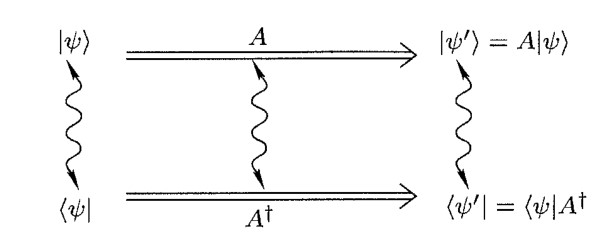
\includegraphics[width=0.9\textwidth]{figure/operation.jpg}
        \caption{左右矢空间算符与态的对应}
        \label{fig:measureoperation}
    \end{figure}
        \begin{remark}
            由于$\hat{A}^\dagger$只在左矢空间中作用,这样不方便的地方在于,我们讨论标量积$\langle\psi_i|\hat{A}^\dagger|\psi_j\rangle$的时候,我们只能理解为$\hat{A}^\dagger$作用于左矢$\langle\psi_i|$上再和$|\psi\rangle$做内积的形式。我们可以人为定义$\hat{A}^\dagger$对右矢空间地作用:
            \begin{equation}\label{equ2:2A}
                (\langle\psi_i|\hat{A}^\dagger)|\psi_j\rangle=\langle\psi_i|(\hat{A}^\dagger|\psi_j\rangle)
            \end{equation}
            上式的意思是,对于给定的右矢$\hat{A}^\dagger|\psi_j\rangle$,总可以和某一个左矢$\langle\psi_i|$形成内积。于是$\hat{A}^\dagger|\psi_j\rangle$是一个确定的内积,从而$\hat{A}^\dagger$是右矢空间的一个确定的算符。同理我们也可以类似的定义$\hat{A}$是左矢空间上一个确定的算符,这样定义的好处在于比较灵活的联络了对偶空间间的算符,从而简化了计算与理解。
        \end{remark}
    \subsection{投影算符}
    本节我们讨论一个量子力学非常常用的一个算符:投影算符。它的引入是基于完备线性空间上任意一个态矢量$|\psi\rangle$都能表示成空间上的一组规范正交基的$\{|\varphi_i\rangle\}$的线性组合,并且展开系数一定为态矢量$|\psi\rangle$到基矢量的投影,即:
    \begin{equation}
        |\psi\rangle=\sum_i\langle\varphi_i|\psi\rangle|\varphi_i\rangle
    \end{equation}
    
    由于$\langle\varphi_i|\psi\rangle$是一个数,因此我们可以将它与$|\varphi_i\rangle$交换位置,可以得到投影算符的定义:
    \begin{equation}
        |\psi\rangle=\sum_i|\varphi_i\rangle\langle\varphi_i|\psi\rangle=\Big(\sum_i|\varphi_i\rangle\langle\varphi_i|\Big)|\psi\rangle=\hat{P}|\psi\rangle
    \end{equation}
    
    如果$\{\varphi_i\}$是一个完备基,那么我们可以将上式看作一个恒等算符$\hat{I}$作用在$|\psi\rangle$上。投影算符的作用是对$|\psi\rangle$在规范正交基$\{\varphi_i\}$下进行投影和分解。
    
    投影算符的一个重要性质就是它的幂等性,即$\hat{P}^2=\hat{P}$:
    \begin{equation}
        \hat{P}^2=\sum_{i,j}|\varphi_i\rangle\langle\varphi_i|\varphi_j\rangle\langle\varphi_j|=\sum_{i,j}|\varphi_i\rangle\langle\varphi_j|\delta_{ij}=\sum_i|\varphi_i\rangle\langle\varphi_i|=\hat{P}
    \end{equation}
    
    \subsection{表象}
    在线性代数中,我们知道,如果我们需要具体的量化矢量的变换,我们可以利用建立坐标轴,利用一组数字来代表矢量与算符\footnote{也就是建立同构关系}。而建立坐标轴的过程也就是在线性空间中取一组基的过程。在量子力学中,我们称取一组基叫做取一个表象。假设$|\phi\rangle,|\psi\rangle$可以按照表象$Q$展开:
    \begin{align}
        \begin{split}
            |\phi\rangle=&\sum_i\langle\varphi_i|\phi\rangle|\varphi_i\rangle=\sum_i b_i|\varphi_i\rangle\\
            |\psi\rangle=&\sum_j\langle\varphi_j|\psi\rangle|\varphi_j\rangle=\sum_j c_j|\varphi_j\rangle
        \end{split}
    \end{align}
    
    假设$|\psi\rangle,|\phi\rangle$之间可以用算符$\hat{A}$联系:
    \begin{equation}
        |\phi\rangle=\hat{A}|\psi\rangle
    \end{equation}
    
    于是有:
    \begin{equation}
        \sum_i b_i|\varphi_i\rangle=\sum_j c_j\hat{A}|\varphi_j\rangle
    \end{equation}
    
    等式两边左乘一个$\langle\varphi_i|$,再利用$\langle\varphi_i|\varphi_j\rangle=\delta_{ij}$的性质,我们可以得到:
    \begin{equation}\label{equ2:2B}
        b_i=\sum_j\langle\varphi_i|\hat{A}|\varphi_j\rangle c_j=\sum_i A_{ij}c_j
    \end{equation}
    
    其中$A_{ij}=\langle\varphi_i|\hat{A}|\varphi_j\rangle$。我们得到了展开系数之间的关系,如果我们令展开系数为列向量的话,我们可以将式\ref{equ2:2B}表示成类似矩阵\footnote{这里说类似矩阵是因为矩阵仅仅针对有限维空间,而量子力学所在空间是无穷维的,因此我们可以类比的想}之间的关系了:
    \begin{equation}
        \begin{pmatrix}
            b_1\\
            b_2\\
            \vdots\\
            b_n\\
            \vdots
        \end{pmatrix}=
        \begin{pmatrix}
            A_{11} & A_{12} & \dots & A_{1n} & \dots\\
            \dots&\dots&\dots&\dots&\dots\\
            A_{m1}&A_{m2}& \dots &A_{mn}&\dots\\
            \dots&\dots&\dots&\dots&\dots
        \end{pmatrix}
        \begin{pmatrix}
             c_1\\
            c_2\\
            \vdots\\
            c_n\\
            \vdots
        \end{pmatrix}
    \end{equation}
    
    于是我们可以知道算符$\hat{A}$在表象Q中对应一个矩阵A,矩阵元为$A_{ij}$。
    
    \subsection{表象变换}
    下面我们讨论不同表象间的变换问题。在线性代数中我们已经知道线性空间中基的变换与过渡矩阵相联系相联系。特别的,在复线性空间中,如果两个基都是规范正交基,那么此时的基变换被称作幺正变换,其对应的过度矩阵Q满足关系:
    \begin{equation}
        Q^\dagger Q=QQ^\dagger=I
    \end{equation}
    
    迁移到量子力学的框架中,由于态空间也是一个复内积空间,同时对于某个表象,我们同样可以将每一个态表示成列向量的形式,因此可以想象,态空间$\mathscr{E}$中的变换也是满足幺正变换的,本节我们验证这个命题。
    
    假设态矢量$|\psi\rangle$可以用两种表象$|a_i\rangle,|b_i\rangle$展开,则有:
    \begin{align}
        \begin{split}
            |\psi\rangle=&\sum_i\langle a_i|\psi\rangle|a_i\rangle=\sum_i C_i^a|a_i\rangle\\
            |\psi\rangle=&\sum_j\langle b_j|\psi\rangle|b_j\rangle=\sum_j C_j^b|b_j\rangle
        \end{split}
    \end{align}
    
    两式联立,可得:
    \begin{equation}
        \sum_i C_i^a|a_i\rangle=\sum_j C_j^b|b_j\rangle
    \end{equation}
    
    等号两边左乘一个$\langle b_k|$,并且由于正交归一关系:$\langle b_k|b_j\rangle=\delta_{kj}$可得:
    \begin{equation}\label{equ2:2C}
        C_k^b=\sum_i C_i^a\langle b_k|a_i\rangle=\sum_i S_{ki}C_i^a
    \end{equation}
    
    其中:
    \begin{equation}
        S_{ki}=\langle b_k|a_i\rangle
    \end{equation}
    
    式\ref{equ2:2C}同样可以写成矩阵形式:
    \begin{equation}
        C^b=S C^a
    \end{equation}
    
    下面我们验证变换矩阵$S$是否是幺正的,我们的思路是通过向表象$\{|a_i\rangle\},\{|b_i\rangle\}$插入投影算符以构造矩阵元$S_{ij}=\langle b_i|a_j\rangle$:
    
    首先向表象$\{|a_i\rangle\}$的正交归一式子中插入投影算符:
    \begin{equation}
         \delta_{ij}=\langle a_i|a_j\rangle=\sum_k \langle a_i|b_k\rangle\langle b_k|a_j=\sum_k S_{ik}^*S_{kj}
    \end{equation}
 
    其矩阵形式为:
    \begin{equation}
        S^\dagger S=I
    \end{equation}
    
    同理,如果我们向表象$\{|b_i\rangle\}$的正交归一式子中插入投影算符,我们可以类似得到:
     \begin{equation}
        S S^\dagger=I
    \end{equation}

   随后我们讨论算符的幺正变换,即对于表象L和表象Q,算符$\hat{A}$对应的矩阵元形式分别为:$A_{ij}=\langle v_i|\hat{A}|v_j\rangle,A_{\alpha\beta}=\langle w_\alpha|\hat{A}|w_\beta\rangle$,如果表象L和表象Q的基底满足某个幺正变换,对应的矩阵用$U$来表示,则对应矩阵元的变换关系为:
   \begin{equation}
       \langle v_i|\hat{A}|v_j\rangle =\sum_\alpha\sum_\beta \langle v_i|w_\alpha\rangle\langle w_\alpha|\hat{A}|w_\beta\rangle\langle w_\beta|v_j\rangle=\sum_\alpha\sum_\beta U^\dagger_{i\alpha}A_{\alpha\beta}U_{\beta j}
   \end{equation}
   
   我们可以将其看作三个矩阵的相乘($A'=U^\dagger$),同理,我们可以采用相同的方法进行反表示:
   \begin{equation}
        \langle w_\alpha|\hat{A}|w_\beta\rangle=\sum_i\sum_j U_{\alpha i}A_{ij}U^\dagger_{j\beta}
   \end{equation}
   
   由上面的表述,我们可以很容易验证表现变换不改变内积$\langle\psi|\varphi\rangle$以及矩阵元的值$\langle\psi|\hat{A}|\varphi\rangle$。这与我们的物理图像相符。
\section{态空间中物理量的表征}
    \subsection{测量}
        \subsubsection{测量的基本性质}
        本节我们讨论如何表征态空间$\mathscr{E}$中的物理量。在日常生活\footnote{特指用经典力学分析的情况}中,如果想要知道一些宏观物理量,比如体系的位移、温度、压强,最朴素的获得方法就是通过一台对应的一起对待测体系进行测量,如光电门测量位移、温度计测温度、压强计测压强等。根据上面的经验,我们可以归纳出测量的大概定义:即将待测体系与一个满足经典力学规律的仪器相互作用后得到对应物理量的过程。
        
        当一个经典仪器作用到被观测的量子客体上的时候,我们称之为一次“操作”(operation)。我们的目的是要标志该客体状态一些可观测物理量的数值。这里分为两种情况:第一种情况是在做了第一次测量以后,仪器能够给出确定的度数,但是使用同样的仪器再测量第二次、第三次测量,给出的度数和第一次度数可能相等也可能不同,这种测量被称为第一类测量;第二种情况与第一类测量不同,在第一次测量以后,再用相同的仪器对同一客体做第二次测量、第三次测量时,仪器的读数总是百分百完全相同。第二类测量又被称为可预测的(predictable),是量子力学中"一次测量"的准确含义。换句话说,第二类测量给出的读数标志一个量子客体状态的一个力学量。
        
        我们可以这样理解:对于一个态的某一种力学量的测量,连续两次都给出同一数值,也就说测量以后态不发生改变。对于态空间$\mathscr{E}$中的某个态$|\psi\rangle$,如果我们想要进行物理量A的测量,同时测量结果为a,我们可以用本征方程来形容这个测量的过程:
        \begin{equation}
            \hat{A}|\psi\rangle=a|\psi\rangle
        \end{equation}
        
        自然的,我们称态$|\psi\rangle$为力学量$\hat{A}$的一个本征态,对应的数值称为它的一个本征值。特别的,如果一个本征值对应多个本征函数,则称本征值对应的本征函数是简并的;简并的本征函数的个数称为简并度;如果一个本征值对应一个本征函数,我们称该本征值对应的本征函数是非简并的。
        
        下面思考一个问题:之前引入波函数的时候,根据实际需要规定了单值、连续、有限三个性质,那么在这里我们将测量定义为了对应的算符,那么算符有什么限制呢?
        
        从上面的叙述中,我们知道测量与经典仪器的相互作用有关,为了得到更加普遍的结论,我们希望能够略去经典仪器本身的性质与限制(如精度,量程)。因此我们假设对于某一个量子客体的一个力学量A测量所得到的读数全体$\{a_n\}$应该穷尽所有的可能值;换句话说,态空间$\mathscr{E}$上的任意一个态能被力学量A对应的所有本征态线性表示,因此一定有关系:
        \begin{equation}
            |\psi\rangle=\sum_i c_i|\psi_i\rangle\xrightarrow{\hat{A}}\hat{A}|\psi\rangle=\sum_i c_ia_n|\psi_i\rangle
        \end{equation}
        
        需要说明的是,上面两式和测量时发生的塌缩是没有关系的,引入它们的本质是量子力学的态叠加原理。从物理上来讲,当许多个量子客体在相同的初始条件下被制备出来以后,人们对其逐一地进行力学量A地测量,原则上会得到不同的读数,我们自然希望知道不同读数之间有没有关联。在波函数公设中,我们了解到波函数的物理意义是有统计意义的,于是我们可以类似提出测量公设:
        \begin{definition}{测量公设}{measurement}
            对于物理量A,一定存在一个对应的测量算符$\hat{A}$,使得A的所有可取值都是$\hat{A}$本征方程的本征值集$\{a_i\}$
            \begin{equation}
                 \hat{A}|\psi_i\rangle=a_i|\psi_i\rangle
            \end{equation}
            并且其对应的本征态的集合$|\psi_i\rangle$构成态空间上的一组完备基,即:
            \begin{equation}
                |\psi\rangle=\sum_i c_i|\psi_i\rangle
            \end{equation}
            
            其中测量值为$a_i$的概率为:$|\langle \psi_i|\psi\rangle|^2$
        \end{definition}
        
        如果我们考虑简并态的话,假设测量值为$a_i$对应的简并度为$g_i$,那么测量到$a_i$的概率应该为塌缩到对应本征子空间本征函数的概率之和,即:$\sum_i^{g_i}|\langle\psi_{j=1}^{g_i}|\langle\psi_{i=1}^j|\psi\rangle^2$
        \subsubsection{测量的统计性质}
        值得一提的是,测量假设需要用到统计的思想进行诠释。从操作的层面上来讲,如果我们采用频率逼近的方式,即同时测量很多个同一个本征态N次,当$N\rightarrow \infty$时,我们知道测量物理量A的概率会收敛到某一个确定的值上:
        \begin{equation}
            \frac{N(a)}{N}\rightarrow P(a)
        \end{equation}
        
        在$|\psi\rangle$态中,我们定义$\langle A\rangle$为测量N次以后所得到测量值的平均值。根据定义,测量的平均值应该等于测量值的加权:
        \begin{equation}
            \langle \hat{A} \rangle=\frac{1}{N}\sum_n a_n N(a_n)
        \end{equation}
        
        当$N\rightarrow \infty$时,平均值趋于一个确定的值:
        \begin{equation}
             \langle \hat{A} \rangle=\sum_n a_n P(a_n)
        \end{equation}
        
        而根据公设$\ref{def:measurement}$,我们可以知道,如果对于简并本征态集$\{|\psi_n^i\rangle\}$ $P(a_n)$可以被表达为:
        \begin{equation}
            P(a_n)=\sum_{i=1}^{g_n}\langle\psi|\psi_n^i\rangle\langle \psi_n^i|\psi\rangle
        \end{equation}
        
        代入可得:
        \begin{equation}
             \langle \hat{A} \rangle=\sum_n a_n \Big(\sum_{i=1}^{g_n}\langle\psi|\psi_n^i\rangle\langle \psi_n^i|\psi\rangle\Big)
        \end{equation}
        
        代入本征方程:$\hat{A}|\psi_n^i\rangle=a_n|\psi_n^i\rangle$,可以得到:
        \begin{equation}
            \langle \hat{A} \rangle=\sum_n  \sum_{i=1}^{g_n}\langle\psi|\hat{A}|\psi_n^i\rangle\langle \psi_n^i|\psi\rangle
        \end{equation}
        
        由于本征态集$\{|\psi_n^i\rangle\}$是一个正交归一集,于是一定有封闭性关系:
        \begin{equation}
            \sum_n\sum_{i=1}^{g_n}|\psi_n^i\rangle\langle \psi_n^i|=\hat{I}
        \end{equation}
        
        于是可以得到:
        \begin{equation}
            \langle \hat{A}\rangle=\langle\psi|\hat{A}|\psi\rangle
        \end{equation}
        
        我们由此得到了测量值平均值的表达式,这有助于我们判断态矢量的性质。
        
        测量的标准除了准确度以外还有精确度,前者我们往往使用平均值(或称为期望)描述,而后者我们往往使用标准差描述。在测量中,由于算符的不对易,导致物理量的测量常常会相互干扰,因此我们常常考虑多个物理量标准差之间的关系\footnote{这里的内容要用到下一节中测量算符是厄密算符的性质,可以跳过想看下一节再回过头来理解}。首先我们考虑对$|\psi\rangle$态进行力学量A的测量所产生的标准差$\sigma_A^2$:
        \begin{align}
            \begin{split}
             \sigma_A^2=&\left\langle(\hat{A}-\langle\hat{A}\rangle)^2 \right\rangle\\
                =& \langle\psi|(\hat{A}-\langle\hat{A}\rangle)^2|\psi\rangle\\
                =&\langle(\hat{A}-\langle\hat{A})\psi|(\hat{A}-\langle\hat{A})\rangle|\psi\rangle\\
                =&\langle f|f\rangle
            \end{split}
        \end{align}
            
       其中$|f\rangle=(\hat{A}-\langle\hat{A})\rangle|\psi\rangle$。同样的方法,对$|\psi\rangle$态进行力学量B的测量所产生的标准差$\sigma_B^2$为:
       \begin{equation}
           \sigma_B^2=\langle g|g\rangle
       \end{equation}
       
       其中:$|g\rangle=(\hat{B}-\langle\hat{B}\rangle)|\phi\rangle$。
       
       我们通过Cauchy-Schwarz不等式,可以建立两个力学量标准差的关系:
       \begin{equation}
           \sigma_A^2\sigma_B^2=\langle f|f\rangle\langle g|g\rangle\geq (\langle f|g\rangle)^2
        \end{equation}

        随后对$\langle f|g\rangle$进行估计,由于这个标量积的结果一定是个复数,而对于任意的复数$z$,一定有以下缩放不等式:
        \begin{equation}
            z=Rez+Imz\geq Imz=\frac{1}{2i}(z-z^*)
        \end{equation}
        
        令$z=\langle f|g\rangle$,则$z^*=\langle g|f\rangle$,代入可得:
        \begin{equation}
            \langle f|g\rangle \geq \frac{1}{2i}(\langle f|g\rangle-\langle g|f\rangle)
        \end{equation}
        
        根据$\langle f|g\rangle$的定义,我们可以得到:
        \begin{align}
            \begin{split}
                \langle f|g\rangle=&\langle\psi|(\hat{A}-\langle\hat{A}\rangle)(\hat{B}-\langle\hat{B}\rangle)|\phi\rangle\\
                =&\langle\psi|(\hat{A}\hat{B}-\langle\hat{A}\rangle\hat{B}-\hat{A}\langle\hat{B}\rangle+\langle\hat{A}\rangle\langle\hat{B}\rangle)|\phi\rangle
            \end{split}
        \end{align}
        
        同理,对于$\langle g|f\rangle$,有\footnote{这里的第二个等号利用了厄米算符矩阵元的定义:$\langle\phi|\hat{A}|\psi\rangle=\langle\psi|\hat{A}|\phi\rangle$,详细证明可以见下一节}:
        \begin{align}
            \begin{split}
                \langle g|f\rangle=&\langle\phi|(\hat{B}\hat{A}-\langle\hat{A}\rangle\hat{B}-\hat{A}\langle\hat{B}\rangle+\langle\hat{A}\rangle\langle\hat{B}\rangle)|\psi\rangle\\
                =&\langle\psi|(\hat{B}\hat{A}-\langle\hat{A}\rangle\hat{B}-\hat{A}\langle\hat{B}\rangle+\langle\hat{A}\rangle\langle\hat{B}\rangle)|\phi\rangle
            \end{split}
        \end{align}
            
        于是代入上述所有式子可以得到一个重要的不等式:
        \begin{equation}
            \sigma_A^2\sigma_B^2\geq \Big(\frac{1}{2i}\langle [\hat{A},\hat{B}]\rangle\Big)^2
        \end{equation}
        
        上式被称为广义的不确定原理,对于每一对不对易的力学量测量算符,都存在这样类似的测不准原理\footnote{关于不对易的力学量测量算符的性质,将在\ref{subsection:ESCO}节中给予详细阐释}。特别的当$\hat{A}=\hat{x},\hat{B}=\hat{p_x}$时,我们知道$[\hat{x},\hat{p_x}]=i\hbar$,代入上式,可以得到$\sigma_x\sigma_{p_x}\geq\frac{\hbar}{4}$。
        
        \begin{remark}
            从上面的表述可以看到,测不准原理并不是量子力学新的假设,而是实验的自然推断,也是量子力学具有统计性质的根源之一。
        \end{remark}
    \subsection{测量算符}
        本节我们继续探讨测量算符具有什么性质。从测量结果的角度来看,对任意一个可观测物理量的测量结果都应该为实数。这一点体现为:对于$\hat{A}$的本征态来说,我们要保证其本征值为实数;对于一般的态$|\psi\rangle$,虽然它的测量结果各有不同,但是由于所有的测量结果都应为实数,因此平均值$\langle\psi|\hat{A}|\psi\rangle$一定为实数,因此$\langle\psi|\hat{A}|\psi\rangle$一定等于其共轭\footnote{这里利用到了标量积的性质:
        \begin{equation*}
            (\langle\psi|\hat{A}|\phi\rangle)^*=( (\langle\psi|\hat{A}\phi\rangle)^*=\langle\hat{A}\phi|\psi\rangle=\langle\psi|\hat{A}^\dagger|\phi\rangle
        \end{equation*}}:
        \begin{equation}
            \langle \psi|\hat{A}|\psi\rangle=(\langle\psi|\hat{A}|\psi\rangle)^*=\langle\psi|\hat{A}^\dagger|\psi\rangle
        \end{equation}
        
        因此测量算符一定满足$\hat{A}=\hat{A}^\dagger$,我们称$\hat{A}$是厄米算符。因此有关测量算符的假设就与厄米算符有关:
        \begin{definition}{算符公设Ⅱ}{measurement2}
            测量算符一定是一个厄米算符。
        \end{definition}
        
        厄米算符还有其它良好的性质。假设$|\phi_1\rangle,|\phi_2\rangle$是测量算符$\hat{A}$不同本征值对应的本征态,即有本征方程:
        \begin{align}
            \begin{split}
                \hat{A}|\phi_1\rangle=a_1|\phi_1\rangle\\
                \hat{A}|\phi_2\rangle=a_2|\phi_2\rangle
            \end{split}
        \end{align}
        
        考虑标量积$\langle\phi_1|\hat{A}|\phi_2$,结合本征方程,可以得到:
        \begin{equation}
            a_1\langle\phi_1|\phi_2\rangle=\langle\phi_1|\hat{A}|\phi_2=a_2\langle\phi_1|\phi_2\rangle
        \end{equation}
        
        由于$a_1\ne a_2$,因此$\langle\phi_1|\phi_2\rangle=0$,也即:厄米算符不同本征值对应的本征态相互正交。这个性质非常重要,对于同一本征值的本征态,我们一定可以通过Gram-Schimdt正交化获得正交归一的本征态集。综上所述,如果算符是Hermitian的,我们一定可以找到一组正交归一的完备基。
    \subsection{可对易观察算符的完全集合(ESCO)}\label{subsection:ESCO}
    本节我们考虑两个对易的观察算符所具有的性质。首先从两个简单的性质出发:
    \begin{theorem}{性质1}{property1}
    如果$[\hat{A},\hat{B}]=0$,则$\hat{A}$的所有本征子空间在$\hat{B}$的作用下不变,即:对于$\hat{A}$的任意本征值$a_n$所对应的本征子空间$\mathscr{E}_{a_n}$,如果$|\psi\rangle\in\mathscr{E}_{a_n}$,则$\hat{B}|\psi\rangle\in\mathscr{E}_{a_n}$
    \end{theorem}
    \begin{proof}
    假设$|\psi\rangle$是算符$\hat{A}$的本征态,本征值为a,则根据对易关系,$\hat{A}\hat{B}=\hat{B}\hat{A}$,有:
    \begin{equation}
        \hat{A}(\hat{B}|\psi\rangle)=\hat{B}\hat{A}|\psi\rangle=a(\hat{B}|\psi\rangle
    \end{equation}
    
    由上式,我们知道$\hat{B}|\psi\rangle$也满足$\hat{A}$的本征方程,故证得
    \end{proof}
    \begin{theorem}{性质2}{property2}
        如果$[\hat{A},\hat{B}]=0$,并且$|\psi_1\rangle,|\psi_2\rangle$是算符$\hat{A}$的两个不同的本征态,并且属于不同的本征值,则$\langle\psi_1|\hat{B}|\psi_2\rangle=0$
    \end{theorem}
    \begin{proof}
    由定理\ref{thm:property1}可得,当$[\hat{A},\hat{B}]$对易的时候,$\hat{B}|\psi_2\rangle\in \mathscr{E}_{a_2}$。根据厄米算符的性质,不同本征值对应的本征态是相互正交的,因此$\langle\psi_1|\hat{B}|\psi_2\rangle=0$
    \end{proof}
    
    根据性质1、性质2,我们可以得到非常重要的性质3:
    \begin{theorem}{性质3}{property3}
        如果观察算符满足$[\hat{A},\hat{B}]=0$,则它们共同本征态构成态空间$\mathscr{E}$上的一组完备正交归一基。
    \end{theorem}
    \begin{proof}
        证明性质3,本质上就是证明一定存在一组规范正交基组$\{v_n^i\}$,使得$\hat{A},\hat{B}$在这组基对应的矩阵是对角矩阵。假设$\{|u_n^i\rangle\}$是$\hat{A}$的一组本征态,则一定满足本征方程:
        \begin{equation}
            \hat{A}|u_n^i\rangle=a_n|u_n^i\rangle,i=1,2\dots,g_n
        \end{equation}
        
        其外,基一定满足正交归一关系:
        \begin{equation}
            \langle u_n^i|u_{n'}^{i'}\rangle=\delta_{ii'}\delta_{nn'}
        \end{equation}
        
        可以看到,此时$\hat{A}$在$\{|u_n^i\rangle\}$下的矩阵是对焦矩阵,那么$\hat{B}$在$\{|u_n^i\rangle\}$下的矩阵形式是怎么样的呢?根据性质2,我们知道B矩阵的矩阵元满足$\langle u_n^i|\hat{B}|u_n^{i'}\rangle=0$,由此可以看出B的形式应该是一个分块对角矩阵,每一个子块是一个$g_n\times g_n$的矩阵(如图\ref{fig:multiblock})
       
        我们分情况讨论。如果$\{|u_n^i\rangle\}$是非简并的,即$g_n=1,n=1,2,\dots$,那么B矩阵就是对角矩阵,此时性质3已经成立;如果如果$\{|u_n^i\rangle\}$是简并的,即$\exists n,g_n\ne1$,此时可以发现$\{|u_n^i\rangle\}$不是$\hat{B}$的本征态。由于$\hat{A}$存在本征方程,也就是说,我们可以使用$\hat{A}$的本征子空间表示态空间$\mathscr{E}$:
        \begin{equation}
            \mathscr{E}=\mathscr{E}_{a_1}\oplus \mathscr{E}_{a_2}\oplus\dots\oplus \mathscr{E}_{a_n}\oplus\dots
        \end{equation}
        
        于是,本征子空间中的任意一组正交归一基都能让A称为对角矩阵。对于B矩阵,由于$\hat{B}$是Hermitian的,因此B矩阵的子块也一定是Hermitian的。根据线性代数的知识,厄米矩阵一定是可以对角化的,因此一定存在正交归一基$\{|v_n^i\rangle\}$,使得:
        \begin{equation}
            \langle v_n^i|\hat{B}|v_n^j\rangle=\delta_{ij}
        \end{equation}
        
        由此简并态的情况也满足性质3,证毕。
        
         \begin{figure}[H]
            \centering
            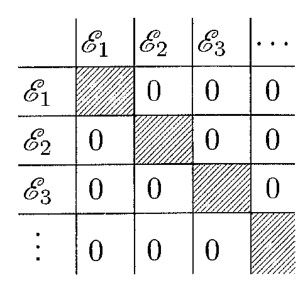
\includegraphics{figure/multiblock.jpg}
            \caption{B矩阵在基$\{|u_n^i\rangle\}$是一个分块对角矩阵}
            \label{fig:multiblock}
        \end{figure}
        
    \end{proof}

性质3提供了对易的观察算符的一个非常好的性质,但是其中有一个细节值得揣摩:能将算符$\hat{B}$对角化后的新的本征态是$\hat{A}$同一本征值下的本征态吗?答案是不一定是。因为在上面的证明中我们仅仅只能保证新的基的存在性,而不能保证新的基与变换前的基与本征值一一对应。这一点看似性质不是很好,但是实际上对于简并情况来说,如果我们测量物理量A,结果为$a_n$,可能存在两个本征态$|\psi_1\rangle,|\psi_2\rangle$满足本征方程,这样从测量的角度上来看我们并不能分辨这两个本征态。此时我们可以通过测量另一个与$\hat{A}$对易的物理量B来分辨这两个状态;换句话说,如果存在一组本征值组$\{a_n,b_p\}$对应唯一的一个态矢量,我们就能够通过测量完全确定一个态;如果本征值组$\{a_n,b_p\}$仍然不能对应唯一一个态矢量,那么我们就引入与$\hat{A},\hat{B}$对易的物理量C,如果存在一组本征值组$\{a_n,b_p,c_r\}$对应唯一一个共同的本征态,那么就可以通过测量完全确定一个态;如果不能,继续引入新的对易算符$\dots$\footnote{其实可以看出,引入对易算符并通过测量的本征值描述态本质上就是回归了经典力学描述状态的方法,我们可以将测量的本征值看作描述状态的自由度}。由此,我们引出了CSCO的概念:
\begin{definition}{CSCO}{CSCO}
    如果测量算符$\hat{A},\hat{B},\hat{C}\dots$相互对易,并且一定存在测量的本征值组$\{a_n,b_p,c_r\}$确定唯一的一个共同本征态,我们将果测量算符$\hat{A},\hat{B},\hat{C}\dots$的集合称为可对易观察算符的完全集合,简写为CSCO。
\end{definition}

对于CSCO,还有几点注意:
\begin{enumerate}
    \item 通常我们只考虑最小的CSCO,如果$\hat{A},\hat{B}$已经构成了CSCO,在一般情况下我们不会考虑继续加一个新的算符$\hat{C}$;
    \item 由于一组本征值组确定唯一一个本征态,因此我们可以将本征态简记为本征值组的形式,如:$|a_n,b_p,c_r\rangle$;
    \item 对于一个给定的态空间,CSCO可能不止一组。
\end{enumerate}

    CSCO还有一个值得讨论的点,就是多个算符在操作上是如何测量的。首先,由于测量以后,在短时间内会发生态的塌缩,但是态在其它时候都是遵循Schrodinger方程的演化\footnote{详细讨论可以见\ref{section2:evolution}节}。因此算符测量见的间隔不能太长;此外测量的先后顺序会不会影响最后的结果呢?答案显然是否定的,在这里我们讨论一种简单的情况,即$\hat{A},\hat{B}$构成CSCO,我们设共同本征态为$|a_n,b_p\rangle$,于是对于态空间上的任意一个态$|\psi\rangle$,我们总是可以表示为:
    \begin{equation}
        |\psi\rangle=\sum_{n,p}c_{n,p}|a_n,b_p\rangle
    \end{equation}
    
    于是根据测量公设,第一次测量物理量A对应的测量值为$a_n$的概率为:
    \begin{equation}
        P(a_n)=\sum_p |c_{n,p}|^2
    \end{equation}
    
    第一次测量后的态从$|\psi\rangle$变为$|\psi'\rangle$\footnote{公式里的n是一个定值而不是变量,可以将其看作投影算符对$|\psi\rangle$的作用,使之从高维空间的矢量压缩成了低维空间的矢量。}:
    \begin{equation}
        |\psi'\rangle=\sum_p c_{n,p}|a_n,b_p\rangle\cdot \frac{1}{\sqrt{\sum_p|c_{n,p}|^2}}
    \end{equation}
    
    其中乘积的第二项是考虑到了态的归一化。此时我们可以获得在第一次测量物理量A的结果为$a_n$的前提下,第二次测量物理量B的结果为$b_p$的条件概率为:
    \begin{equation}
        P(b_p|a_n)=\frac{|c_{n,p}|^2}{\sqrt{\sum_p|c_{n,p}|^2}}
    \end{equation}
    
    于是,根据概率公式,我们可以得到测量结果为$a_n,b_p$的概率为:
    \begin{equation}
        P(a_n,b_p)=P(a_n)P(b_p|a_n)=|c_{n,p}|^2
    \end{equation}
    
    同理,对于先测量物理量B后测量物理量A的情况,我们也能得到同样的结果,因此无论测量是按照何种顺序进行的,物理上的结果都是一样的。但是对于不对易的算符来说就不同了。举一个简单的例子:假设态空间是一个二维的矢量空间,$|u_1\rangle,|u_2\rangle$是$\hat{A}$本征值为$a_1,a_2$的本征态,$|v_1\rangle,|v_2\rangle$是本征值为$b_1,b_2$的本征态。有图可知,$\hat{A},\hat{B}$没有共同的本征态,因此它们是不对易的。现在考虑对态空间中的任意态$|\psi\rangle$分别进行以下两种测量:
    \begin{align}
        \begin{split}
            a_1,b_2:|\psi\rangle\rightarrow|u_1\rangle\rightarrow|v_2\rangle\\
            b_2,a_1:|\psi\rangle\rightarrow|v_2\rangle\rightarrow|u_1\rangle
        \end{split}
    \end{align}

    我们可以看见两种路径都是测量出$a_1,b_2$的结果,但是末态不同,我们考虑两种路径测量的概率:
    \begin{align}
        \begin{split}
            P(a_1,b_2)=&|OH_1|^2\cdot|OK_2|^2\\
            P(b_2,a_1)=&|OH_2|^2\cdot|OK_1|^2
        \end{split}
    \end{align}
    
    显然$P(a_1,b_2)\ne P(b_2,a_1)$。因此不对易的算符是不能同时测量的,因为第二次的测量会失去第一次测量所得到的信息,因为$|v_2\rangle$不是$\hat{A}$的本征态。
    \begin{figure}[H]
        \centering
        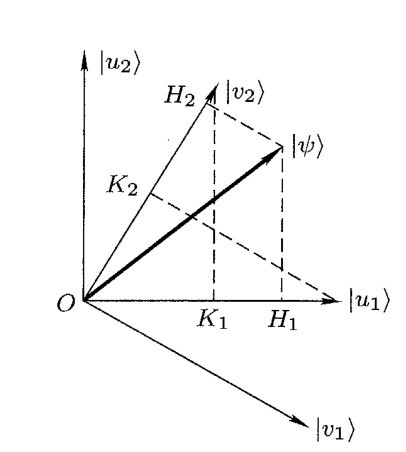
\includegraphics{figure/paradox.jpg}
        \caption{不对易算符不能同时测量}
        \label{fig:noncommuting}
    \end{figure}
\section{态的演化}\label{section2:evolution}
    \begin{definition}{Schrodinger方程公设}{Schrodingerequ}
        态$|\psi(t)\rangle$的演化遵循Schrodinger方程:
        \begin{equation}
            i\hbar\frac{d|\psi(t)\rangle}{dt}=\hat{H}|\psi(t)\rangle
        \end{equation}
        
        其中$\hat{H}$表示与体系能量有关的观察算符,我们称之为Hamiltonian。由于我们观察到这个方程式关于t的一阶微分方程,因此我们只要知道初始条件$|\psi(t_0)\rangle$,状态后续的演化就被唯一的确定
    \end{definition}
    
    本节我们主要从Schrodinger方程出发探讨几个方程的一般性质。
    \subsection{概率守恒}
    本节讨论态的一些统计限制。首先,随着Schrodinger方程的演化,态必须保证还在态空间中,也就是说,需要保证态矢量的归一化不随演化而改变,在数学上我们要证明态的模方$\langle\psi(t)|\psi(t)\rangle$不随时间而改变:
    \begin{equation}\label{equ:D}
        \frac{d}{dt}\langle\psi(t)|\psi(t)\rangle=\frac{d}{dt}\langle\psi(t)|\Big]|\psi(t)\rangle+\langle\psi(t)|\Big[\frac{d}{dt}|\psi(t)\rangle\Big]
    \end{equation}
    
    根据Schrodinger方程,我们可以得到左矢与右矢的导数的表达式:
    \begin{align}\label{equ2:E}
        \begin{split}
            \frac{d|\psi(t)\rangle}{dt}=&\frac{1}{i\hbar}\hat{H}|\psi(t)\rangle\\
            \frac{d\langle\psi(t)|}{dt}=&-\frac{1}{i\hbar}\langle\psi(t)|\hat{H}^\dagger=-\frac{1}{i\hbar}\langle\psi(t)|\hat{H}
        \end{split}
    \end{align}
    
    代入\ref{equ:D}式,可得:
    \begin{equation}
        \frac{d}{dt}\langle\psi(t)|\psi(t)\rangle=0
    \end{equation}
    
    由此我们知道态矢量的归一化不随着演化的改变而改变。事实上,这是一种全空间上的概率守恒;根据电磁学的知识,我们知道一种全局守恒必定对应一种局域守恒。所谓局域守恒,就是对于空间上的任意一个部分,单位时间内“流出”的物理量一定与单位时间内“流入”的物理量相同,其数学形式表现为下列的连续性方程:
    \begin{equation}
        \frac{\partial}{\partial t}\rho(r,t)+\nabla \cdot \Vec{J}=0
    \end{equation}
    
    其中$\rho$是局域空间的密度,$\Vec{J}$被称为该物理量对应的“流”。下面我们证明我们可以从Schrodinger方程推出连续性方程。
    
    由于密度一般来说是时空量,因此我们采用$|r\rangle$表象上的Schrodinger方程较为合适:
    \begin{equation}
        i\hbar\frac{\partial}{\partial t}\psi(r,t)=\Big(\frac{\hat{p}^2}{2m}\nabla^2+V(r,t)\Big)\psi(r,t)
    \end{equation}
    
    其共轭形式为:
    \begin{equation}
        -i\hbar\frac{\partial}{\partial t}\psi^*(r,t)=\Big(\frac{\hat{p}^2}{2m}\nabla^2+V(r,t)\Big)\psi^*(r,t)
    \end{equation}
    
    由于两式右边只有$V(r,t)$有关项是没有偏微分的,因此我们将两式联立消去方程的该部分,可得:
    \begin{align}
        \begin{split}
            i\hbar\Big\{\psi^*(r,t)\frac{\partial}{\partial t}\psi(r,t)+\psi^*(r,t)\frac{\partial}{\partial t}\psi(r,t)\Big\}\\
            =\frac{\hbar^2}{2m}\Big(\nabla^2\psi(r,t)\psi^*(r,t)-\nabla^2\psi^*(r,t)\psi(r,t)\Big)
        \end{split}
    \end{align}
    
    可以看到,等号左边可以根据全微分的计算得到结果为:$i\hbar\frac{\partial}{\partial t}(\psi(r,t)\psi^*(r,t))$,将系数除到等号右边进行化简可以得到:
    \begin{equation}
        i\hbar\frac{\partial}{\partial t}(\psi(r,t)\psi^*(r,t))=\frac{\hbar^2}{2m}\Big(\nabla^2\psi(r,t)\psi^*(r,t)-\nabla^2\psi^*(r,t)\psi(r,t)\Big)
    \end{equation}
    
    我们对等号右侧的式子通过加一项再减一项$\nabla\psi\nabla\psi^*$的方法,可以将右侧凑成一个式子的梯度,于是Schrodinger方程可以写成以下形式:
    \begin{equation}
        i\hbar\frac{\partial}{\partial t}(\psi(r,t)\psi^*(r,t))+\frac{i\hbar}{2m}\nabla[\nabla\psi(r,t)\psi^*(r,t)-\nabla\psi^*(r,t)\psi(r,t)]=0
    \end{equation}
    
    我们定义$\rho=\psi^*\psi$,$\Vec{J}=\frac{i\hbar}{2m}\nabla\psi(r,t)\psi^*(r,t)-\nabla\psi^*(r,t)\psi(r,t)$,就可以将Schrodinger方程转换为连续性方程。我们称此时的$\Vec{J}$为几率流。这个概念在诸如散射问题中有重要的作用。
    \subsection{可观测物理量的演化}\label{subsection:evolutionforoperator}
        在之前的章节中我们已经了解到了可观测物理量平均值满足$\langle\psi(t)|\hat{A}|\psi(t)\rangle$。可以看到,可观测物理量的平均值一方面和态有关,一方面与算符$\hat{A}$有关,而两者都有可能随时间发生变化,因此平均值随时间的演化对于描述算符的演化有重要作用,下面我们详细探讨一下:
        \begin{align}
            \begin{split}
                \frac{d\langle\hat{A}\rangle}{dt}=&\frac{d}{dt}\langle\psi(t)|\hat{A}|\psi(t)\rangle\\
                =&[\frac{d}{dt}\langle\psi(t)|]\hat{A}|\psi(t)\rangle+\langle\psi(t)|\frac{\partial\hat{A}}{\partial t}|\psi(t)\rangle+\langle\psi(t)|\hat{A}|[\frac{d}{dt}|\psi(t)]\\
            \end{split}
        \end{align}
        
        代入式\eqref{equ2:E},可以得到:
        \begin{equation}\label{equ2:evolutionforoperator}
            \frac{d\langle\hat{A}\rangle}{dt}= \langle\frac{\partial\hat{A}}{\partial t}\rangle+\frac{1}{i\hbar}\langle[\hat{A},\hat{H}]\rangle
        \end{equation}
        
        观察该式,我们发现它和经典力学中的Hamilton原理相似,不同的是经典力学中等式右侧第二项是泊松括号,而在量子力学中却变为了对易子。因此经典力学中的泊松括号和量子力学中的对易子是由对应关系的,这个关系最早由Dirac发现,我们将其称为正则量子化,在下一节中,我们将会阐述正则量子化的内容。
        
        \subsection{保守系与定态}
        如果$\hat{H}$不含时间,我们称体系是一个保守系。在经典力学中,如果体系是一个保守系,那么体系的能量守恒,也即能量是一个运动常量。本节我们讨论在量子力学框架下保守系具有的性质。
        
        假设$\hat{H}$满足以下本征方程:
        \begin{equation}
            \hat{H}|\varphi_{n,\tau}\rangle=E_n|\varphi_{n,\tau}\rangle
        \end{equation}
        
        于是,任意时刻t上的态都可以表示为本征态的线性组合:
        \begin{equation}
            |\psi(t)\rangle=\sum_{n,\tau}c_{n,\tau}(t)|\varphi_{n,\tau}\rangle
        \end{equation}
        
        代入Schrodinger方程,可以得到:
        \begin{align}
            \begin{split}
                i\hbar\frac{d}{dt}|\psi(t)\rangle=&\hat{H}|\psi(t)\rangle\\
                =&\hat{H}\Big(\sum_{n,\tau}c_{n,\tau}(t)|\varphi_{n,\tau}\rangle\Big)\\
                =&\sum_{n,\tau}c_{n,\tau}(t)E_n|\varphi_{n,\tau}\rangle
            \end{split}
        \end{align}
        
        用$\langle\varphi_{n,\tau}|$作用于上式,可以得到:
        \begin{align}
            \begin{split}
                i\hbar\frac{d}{dt}\langle \varphi_{n,\tau}|\psi(t)\rangle=&c_{n,\tau}E_n\\
                \Rightarrow i\hbar\frac{dc_{n,\tau}}{dt}=&c_{n,\tau}E_n
            \end{split}
        \end{align}
        
        这是一个简单微分方程,结果为:
        \begin{equation}
            c_{n,\tau}(t)=c_{n,\tau}(t_0)e^{-\frac{iE_n(t-t_0)}{\hbar}}
        \end{equation}
        
        则任意时刻的态$|\psi(t)\rangle$可以表示为:
        \begin{equation}
            |\psi(t)\rangle=\sum_{n,\tau}c_{n,\tau}(t_0)e^{-\frac{iE_n(t-t_0)}{\hbar}}|\varphi_{n,\tau}\rangle
        \end{equation}
        
        我们也可以将其拓展到连续基的情况:
        \begin{equation}
            |\psi(t)\rangle=\sum_{\tau}\int dE c_{E,\tau}(t_0)e^{-\frac{iE_n(t-t_0)}{\hbar}}|\varphi_{E,\tau}\rangle
        \end{equation}
        
        特别的,如果$|\psi(t_0)\rangle$也是$\hat{H}$的本征态,那么:
        \begin{equation}
            |\psi(t_0)\rangle =\sum_{n,\tau}c_{n,\tau}(t_0)|\varphi_{n,\tau}\rangle
        \end{equation}
        
        于是任意时刻的态可以表示为:
        \begin{equation}
            |\psi(t)\rangle=\sum_{n,\tau}c_{n,\tau}(t_0)e^{-\frac{iE_n(t-t_0)}{\hbar}}|\varphi_{n,\tau}\rangle=e^{-\frac{iE_n(t-t_0)}{\hbar}}|\psi(t_0)\rangle
        \end{equation}
        
        可以发现任意时刻的态与$t_0$时刻的态相比仅仅多了一个总的相位因子,根据上文的讨论,我们知道两个态的物理性质完全相同,即处在$\hat{H}$的本征态的所有可观测物理量的取值都不随时间变化,因此我们称之为定态。这是后续我们处理问题的立足点。
        
    %能量-时间不确定关系+光谱带宽    
\section{$|r\rangle$和$|p\rangle$表象}
    本节介绍常用的两个表象:$|r\rangle$和$|p\rangle$表象,用来复习第二章的主要脉络,同时这两个表象与经典力学的联系十分紧密,我们可以在后文看到一些有趣的结论
    \subsection{基的基本性质}
    通过扩充态空间$\mathscr{E}$,使得在实际操作上可以取所谓的连续基$\{\omega_\alpha\}$。下面介绍两个典型的连续基,一个是与$r$有关的$\delta$函数,一个是平面波函数,我们分别用$|r_0\rangle,|p_0\rangle$表示:
    \begin{align}
        \begin{split}
            |r_0\rangle=&\delta(r-r_0)=\xi_{r_0}(r)\\
            |p_0\rangle=&(2\pi\hbar)^{-\frac{3}{2}}\exp{\frac{ip_0\cdot r}{\hbar}}=v_{p_0}(r)
        \end{split}
    \end{align}
    
    虽然这两组基不在态空间内,但是态空间内的所有态都可以用它们表示。因此从这两个连续基出发,定义两种表象$|r\rangle,|p\rangle$。前者由x,y,z三个连续指标描述,后者由$p_x,p_y,p_z$三个连续指标描述。下面验证两组基的基本性质。首先根据态空间上标量积的定义,容易验证:
    \begin{align}
        \begin{split}
            \langle r_0|r_0'\rangle=&\int d^3r\xi^*_{r_0}(r)\xi_{r_0'}(r)=\delta(r_0-r_0')\\
            \langle p_0|p_0\rangle=&\int d^3p v^*_{p_0}(r)v_{p_0'}(r)=\delta(p_0-p_0')
        \end{split}
    \end{align}
    
    因此两种表象都是正交归一的,同时它们也满足封闭性:
    \begin{align}
        \begin{split}
            \int d^3 r_0|r_0\rangle\langle r_0|=1\\
            \int d^3 p_0 |p_0\rangle\langle p_0|=1
        \end{split}
    \end{align}
    
    将投影算符作用到态空间上的态$|\psi\rangle$上,可以得到:
    \begin{align}
        \begin{split}
            |\psi\rangle=&\int d^3 r_0|r_0\rangle\langle r_0|\psi\rangle\\
            |\psi\rangle=&\int d^3 p_0|p_0\rangle\langle p_0|\psi\rangle
        \end{split}
    \end{align}
    
    其中展开系数可以这样表示:
    \begin{align}
        \begin{split}
            \langle r_0|\psi\rangle=&\int d^3 r\xi_{r_0}^*(r)\psi(r)=\psi(r_0)\\
            \langle p_0|\psi\rangle =& \int d^3p v_{p_0}^*(r)\psi(r)=\overline{\psi(p_0)}
        \end{split}
    \end{align}
    
    因此,波函数$\psi(r_0)$代表态在表象$|r\rangle$上对应$|r_0\rangle$的坐标。同理,$\overline{\psi(p_0)}$也有类似的解释。
    \subsection{$|r\rangle$到$|p\rangle$的表象变换}
        本节主要讨论$\psi(r)$与$\overline{\psi(p)}$的关系,首先考虑标量积$\langle r|p\rangle$:
        \begin{equation}
            \langle r|p\rangle=v_p(r)=(2\pi\hbar)^{-\frac{3}{2}}\exp{\frac{ip\cdot r}{\hbar}}
        \end{equation}
        
        插入封闭关系式可以得到:
        \begin{align}
            \begin{split}
                \psi(r)=\langle r|\psi\rangle=&\int d^3 p\langle|p\rangle\langle p|\psi\rangle =(2\pi\hbar)^{\frac{3}{2}}\int d^3 p\exp{\frac{ip\cdot r}{\hbar}}\overline{\psi(p)}\\
                \overline{\psi(p)}=\langle p|\psi\rangle=&\int d^3 r\langle p|r\rangle\langle r|\psi\rangle=(2\pi\hbar)^{-\frac{3}{2}}\int d^3r\exp{\frac{ip\cdot\psi(r) r}{\hbar}}
            \end{split}
        \end{align}
        
        可以明显发现,两者满足Fourier变换。下面我们讨论可观测量的表象变换,考虑算符$\hat{A}$在$|r\rangle$表象下的矩阵元$\langle r'|\hat{A}|r\rangle$,我们通过插入两个封闭关系构造$\hat{A}$在$|p\rangle$表象下的矩阵元$\langle p'|\hat{A}|p\rangle$:
        \begin{align}
            \begin{split}
                \langle r'|\hat{A}|r\rangle=&\int d^3p'\langle r'|p'\rangle\int d^3p\langle p'|\hat{A}|p\rangle\langle p|r\rangle
                \\=&(2\pi\hbar)^{-3}\int d^3p'\langle r'|p'\rangle\int d^3p \exp{\frac{i(p'-p)\cdot r}{\hbar}}\langle p'|\hat{A}|p\rangle
            \end{split}
        \end{align}
    \subsection{观察算符$\hat{R}$和$\hat{P}$}
        本节我们讨论观察算符$\hat{R}$和$\hat{P}$的性质,我们假设态空间上存在与x方向有关的变换:
        \begin{equation}
            |\psi'\rangle=\hat{X}|\psi\rangle
        \end{equation}
        
        在$|r\rangle$表象下,根据测量算符的性质,我们知道一定有关系:
        \begin{equation}
            \langle r|\psi'\rangle=\langle r|\hat{X}|\psi\rangle= x\langle r|\psi\rangle
        \end{equation}
        
        同理:
        \begin{align}
            \begin{split}
                \langle r|\hat{Y}|\psi\rangle= y\langle r|\psi\rangle\\
                \langle r|\hat{Z}|\psi\rangle= z\langle r|\psi\rangle
            \end{split}
        \end{align}
        
        这里的$x,y,z$是标记$|r\rangle$的三个指标,因此我们可以将$\hat{X},\hat{Y},\hat{Z}$理解为算符$\hat{R}$的三个分量。上述定义给计算$|r\rangle$表象下的一些物理量提供了方便,比如平均值$\langle \hat{X}\rangle$:
        \begin{equation}
            \langle \hat{X}\rangle=\langle\psi|\hat{X}|\psi\rangle=\int d^3r\langle\psi|r\rangle\langle r|\hat{X}|\psi\rangle=\int d^3r\psi^*(r)x\psi(r)
        \end{equation}
 
        同理,我们可以定义态空间中有关动量的测量算符$\hat{P_x},\hat{P_y},\hat{P_z}$:
        \begin{align}
            \begin{split}
                \langle p|\hat{P_x}|\psi\rangle=&p_x\langle p|\psi\rangle\\
                p|\hat{P_y}|\psi\rangle=&p_y\langle p|\psi\rangle\\
                p|\hat{P_z}|\psi\rangle=&p_z\langle p|\psi\rangle
            \end{split}
        \end{align}
        
        下面我们思考一个重要的例子:$\hat{P}$算符在$|r\rangle$表象下的情况:
        \begin{equation}
            \langle r|\hat{P_x}|\psi\rangle=\int d^3p\langle r|p\rangle\langle p|\hat{P_x}|\psi\rangle =\int d^3p\langle r|p\rangle p_x\langle p|\psi\rangle=(2\pi\hbar)^{-\frac{3}{2}}\int d^3p e^{\frac{ip\cdot r}{\hbar}}p_x\overline{\psi(p)}
        \end{equation}
        
        由上式,我们知道$\langle r|\hat{P_x}|\psi\rangle$应该对应$p_x\overline{\psi(p)}$的逆Fourier变换。可以想到,逆Fourier变换后的结果与$\psi(r)$有关。因此考虑$\psi(r)$的Fourier变换:
        \begin{align}
            \begin{split}
                \psi(r)=& \langle r|\psi\rangle\\
                =&\int d^3 p\langle|p\rangle\langle p|\psi\rangle\\
                =&(2\pi\hbar)^{\frac{3}{2}}\int d^3 p\exp{\frac{ip\cdot r}{\hbar}}\overline{\psi(p)}
            \end{split}
        \end{align}
            

        我们发现等号右边只有指数项$\exp{\frac{ip\cdot r}{\hbar}}$含有r,如果我们对该式对x求偏导数,那么就会在指数项前产生$p_x$并且不改变指数项本身:
        \begin{equation}
            \frac{\partial}{\partial x}\psi(r)= \langle r|\psi\rangle=\int d^3 p\langle|p\rangle\langle p|\psi\rangle =(2\pi\hbar)^{\frac{3}{2}}\int d^3 p\exp{\frac{ip\cdot r}{\hbar}}\Big(\frac{i}{\hbar}p_x\Big)\overline{\psi(p)}
        \end{equation}
        
        如果用$F[\psi(r)]=\overline{\psi(p)}$表示Fourier变换关系的话,那么上式可以简记为:
        \begin{equation}
            F\Big(\frac{\partial}{\partial x}\psi(r)\Big)=\frac{i}{\hbar}p_x\overline{\psi(p)}
        \end{equation}
        
        那么$p_x\overline{\psi(p)}$Fourier逆变换应该为:
        \begin{equation}
            p_x\overline{\psi(p)}=F^{-1}\Big(\frac{\hbar}{i}\frac{\partial}{\partial x}\psi(r)\Big)
        \end{equation}
        
        于是:
        \begin{equation}
            \langle r|\hat{P_x}|\psi\rangle=\frac{\hbar}{i}\frac{\partial}{\partial x}\psi(r)=\Big(\frac{\hbar}{i}\frac{\partial}{\partial x}\Big)\langle r|\psi\rangle
        \end{equation}

        同理$\hat{P_y},\hat{P_z}$有类似的形式,我们可以用$\hat{P}$总结为下式\footnote{$|\psi\rangle$是任意态}:
        \begin{equation}
            \langle r|\hat{P}|\psi\rangle=\frac{\hbar}{i}\nabla\cdot\langle r|\psi\rangle
        \end{equation}
        
        根据上式,我们可以计算在$|r\rangle$表象中与$\hat{P}$算符有关的物理量:
        \begin{equation}
            \langle \hat{P}\rangle=\langle \psi|\hat{P}|\psi\rangle=\int d^3 r\psi^*(r)\Big(\frac{\hbar}{i}\nabla\Big)\cdot \psi(x)
        \end{equation}
        
        然后我们讨论$\hat{X}$与$\hat{P_x}$的对易子在$|r\rangle$表象下的表达式:
        \begin{align}
            \begin{split}
                \langle r|[\hat{X},\hat{P_x}]|\psi\rangle=&\langle r|\hat{X}\hat{P_x}-\hat{P_x}\hat{X}|\psi\rangle\\
                =&x\langle r|\hat{P_x}|\psi\rangle-\Big(\frac{\hbar}{i}\frac{\partial}{\partial x}\Big)\langle r|\hat{X}|\psi\rangle\\
                =&x\Big(\frac{\hbar}{i}\frac{\partial}{\partial x}\Big)\langle r|\psi\rangle-\Big(\frac{\hbar}{i}\frac{\partial}{\partial x}\Big)[x\langle r|\psi\rangle]\\
                =&i\hbar\langle r|\psi\rangle
            \end{split}
        \end{align}
        
        由于$|\psi\rangle$是任意的,因此我们有:
        \begin{equation}
            [\hat{X},\hat{P_x}]=i\hbar
        \end{equation}
        
        其它情况同理,我们总结为下面的三个式子:
        \begin{align}\label{equ2:quantumize}
            \begin{split}
                [\hat{R_i},\hat{R_j}]=&0\\
                [\hat{P_i},\hat{P_j}]=&0\\
                [\hat{R_i},\hat{P_j}]=&i\hbar\delta_{ij}
            \end{split}
        \end{align}
        
        其中$\hat{R_1},\hat{R_2},\hat{R_3}$分别代表$\hat{X},\hat{Y},\hat{Z}$;$\hat{P_1},\hat{P_2},\hat{P_3}$分别代表$\hat{P_x}\hat{P_y}\hat{P_z}$ 。上式被称为正则对易关系,这个关系在量子力学中具有非常重要的地位。
    \subsection{正则量子化}
    基于正则对易关系,我们可以给出一般的可观测物理量$\mathscr{A}$算符化的方法。在上一节的内容中,我们知道与位移$\Vec{r}$和动量$\Vec{p}$对应的观察算符分别为$\hat{R},\hat{P}$,同时它们之间满足\eqref{equ2:quantumize}式的正则对易关系。对于处于标量场作用下无自旋粒子体系的可观测物理量$\mathscr{A}$,我们都可以用基本物理量表示,即:
    \begin{equation}
        \mathscr{A}=\mathscr{A}(\Vec{r},\Vec{p},t)
    \end{equation}
    
    要得到观察算符$\hat{A}$,我们可以简单的用观察算符$\hat{R},\hat{P}$代替变量$\Vec{r},\Vec{p}$,即:
    \begin{equation}
        \hat{A}=\hat{A}(\hat{R},\hat{P},t)
    \end{equation}
    
    举一个简单的例子:考虑一个质量为m,电荷为q,处于标量势场V(R)下的无自旋粒子,其哈密顿量可以写作:
    \begin{equation}
        \mathscr{H}=\frac{p^2}{2m}+V(R)
    \end{equation}
    
    根据上述量子化的规则,Hamiltonian可以简单表示为:
    \begin{equation}
        \hat{H}=\frac{\hat{P}^2}{2m}+V(R)
    \end{equation}
    
    但是这样简单的定义会存在问题,比如如果物理量中含有标量积$\Vec{r}\cdot \Vec{p}$,在经典力学中该标量积是对易的,即:
    \begin{equation}
        r\cdot p=xp_x+yp_y+zp_z=p\cdot r
    \end{equation}
    
    但是由于正则对易关系\eqref{equ2:quantumize}式,我们可以知道算符并不满足对易关系:
    \begin{equation}
        \hat{R}\cdot\hat{P}\ne \hat{P}\cdot\hat{R}
    \end{equation}
    
    同时$\hat{R}\cdot\hat{P}$也不是Hermitian,这将会给量子力学的建立带来很大的麻烦:
    \begin{equation}
        (\hat{R}\cdot\hat{P})^\dagger=\hat{P}\cdot\hat{R}\ne\hat{R}\cdot\hat{P}
    \end{equation}
    
     因此为了使这一类算符构造能够满足对易性和厄密性,我们增加了一条对称性假定,如$\Vec{r}\cdot\Vec{p}$,我们构造成:
     \begin{equation}
         \frac{1}{2}(\hat{R}\cdot\hat{P}+\hat{P}\cdot\hat{R})
     \end{equation}
     
     通过简单的验证,上述算符显然满足对易性和厄密性,遇到更复杂的算符形式也用类似的方法构造。此外,基于非相对论量子力学,有一些算符的建立是不急于上述逻辑的(比如自旋),是通过引入额外的假设来使我们的理论符合实验。
    \subsection{Ehrenfest定理}
    本节对应\eqref{subsection:evolutionforoperator}节中的\eqref{equ2:evolutionforoperator}式。我们知道,位移算符$\hat{R}$和动量算符$\hat{H}$都是不随时间改变的算符,即$\frac{\partial\hat{R}}{\partial t}=\frac{\partial\hat{P}}{\partial t}=0$,因此\eqref{equ2:evolutionforoperator}可以有以下关系:
    \begin{align}
        \begin{split}
            \frac{d\langle \hat{R}\rangle}{dt}=&\frac{1}{i\hbar}\langle[\hat{R},\hat{H}]\rangle=\frac{1}{i\hbar}[\hat{R},\frac{\hat{P}^2}{2m}]\\
            \frac{d\langle \hat{P}\rangle}{dt}=& \frac{1}{i\hbar}\langle[\hat{P},\hat{H}]\rangle=\frac{1}{i\hbar}\langle[\hat{P},V(\hat{R})]\rangle
        \end{split}
    \end{align}
    
    第一式相对容易解,利用对易子的计算性质和基本对易关系:$[\hat{R},\hat{P}]=i\hbar$,我们可以得到:
    \begin{equation}
        [\hat{R},\frac{\hat{P}^2}{2m}]\frac{1}{2m}\Big(\hat{P}[\hat{R},\hat{P}]+[\hat{R},\hat{P}]\hat{P}\Big)=\frac{i\hbar}{m}\hat{P}
    \end{equation}
    
    于是:
    \begin{equation}
         \frac{d\langle \hat{R}\rangle}{dt}=\frac{\langle\hat{P}\rangle}{m}
    \end{equation}
   
   第二式求解对易子$[\hat{P},V(\hat{R})]$相对困难,我们可以以一种更为直观的方法计算,即我们可以认为$V(\hat{R})$一定可以展开成$\hat{R}$的幂级数形式\footnote{不纠结级数收敛的问题,只是一种理解方法}:
   \begin{equation}
       V(\hat{R})=\sum_n c_n \hat{R}^n
   \end{equation}
   
   由此问题转化为求对易子$[\hat{P},\hat{R}^n]$的形式,用数学归纳法不难得到:
   \begin{equation}
       [\hat{P},\hat{R}^n]=-i\hbar n[\hat{P},\hat{R}^n-1]
   \end{equation}
   
   于是:
   \begin{equation}
       [\hat{P},V(\hat{R})]=-i\hbar \nabla V(\hat{R})
   \end{equation}
   
   综上所述,我们可以得到\eqref{equ2:evolutionforoperator}式的两种特殊情况:
   \begin{align}\label{equ2:Erhrenfest}
       \begin{split}
           \frac{d\langle \hat{R}\rangle}{dt}=&\frac{\langle\hat{P}\rangle}{m}\\
           \frac{d\langle \hat{P}\rangle}{dt}=&-\langle V(\hat{R})\rangle
       \end{split}
   \end{align}
   
   上述形式让我们回想起经典力学中单粒子的Hamilton-Jacobi方程:
   \begin{align}
       \frac{d}{dt}r=&\frac{1}{m}p\\
       \frac{d}{dt}p=&-\nabla V(r)
   \end{align}
   
   从中我们再一次可以看到量子力学与经典力学之间的对应关系。下面我们更进一步讨论Erhrenfest定理的物理意义。从波的角度,我们可以将波函数看作平面波的叠加,即一个波包,于是我们可以将$\langle\hat{R}\rangle$理解为波包的中心,那么各个时刻波包中心的集合称为波包中心走过的轨道。当然严格来说,波包本身不存在轨道,因为波包本身具有宽度,但是如果波包的宽度远远小于我们想要求解的其它物理量的尺度,那么我们可以用波包中心的运动近似地代替波包的运动。在这种近似情况下,量子力学与经典力学描述运动的方式应该是一致的。
   
   从式子上来看,我们将\eqref{equ2:Erhrenfest}式联立,可以得到:
   \begin{equation}
       m\frac{d^2\langle\hat{R}\rangle}{dt^2}=-\langle\nabla V(\hat{R})\rangle
   \end{equation}
   
   可以发现,等式的左端$m\frac{d^2\langle\hat{R}\rangle}{dt^2}$可以理解为作用在波包中心的经典力:
   \begin{equation}
       F_{classical}=m\frac{d^2\langle\hat{R}\rangle}{dt^2}=-\nabla \left.V(r)\right|_{r=\langle R\rangle}
   \end{equation}
   
   如果$\nabla \left.V(r)\right|_{r=\langle R\rangle}=\langle\nabla V(\hat{R})\rangle$,则量子力学与经典力学描述运动的方式是一致的。但是一般说来,平均值的函数值不等于函数的平均值(一个最简单的例子:$f(x)=x^2,x\in[1,2]$,$f(1.5)=2.25$,但是$\frac{f(1)+f(2)}{2}=2.5$,两者并不相等)。
   
   但是如果波包很狭窄,那么两者的差距可以忽略。为了更清晰的分析,我对$\langle \nabla V(\hat{R})$取$|r\rangle$表象:
   \begin{equation}
        \langle \nabla V(\hat{R})\rangle=\int d^3r \psi^*(r,t)[\nabla V(r)]\psi(r,t)=\int d^3r|\psi(r,t)|^2\nabla V(r)
   \end{equation}
   
   如果波包很狭窄,那么$|\psi(r,t)|^2$发生明显变化的尺度远远小于$V(r)$发生明显变化的尺度,即在$\langle\hat{R}\rangle$附近$|\psi(r,t)|^2$的值几乎没有变化,因此我们可以近似认为$\nabla \left.V(r)\right|_{r=\langle R\rangle}\cong\langle\nabla V(\hat{R})\rangle$。我们将这种近似称为准经典近似,这种近似非常重要,因为它告诉我们宏观体系在某种极限下,可以从Schrodinger方程推导出Newton方程。
\section{概率幅与测量拾遗}
这个部分主要讲述我看不同量子力学书籍,各种blog和笔记中与测量和概率幅有关的内容,常记常新,小节与小节之间并没有什么关联。
    \subsection{叠加原理与统计混合的不同}
    本节我们讨论叠加原理。在本笔记中,叠加原理是一个新的术语,你可以将其理解为一组基张成某个线性空间的充分必要条件。因此无论在波函数假设中,还是在Schrodinger方程中,都已经暗藏有叠加原理的性质了。叠加原理的核心有两条:
    \begin{itemize}
        \item 如果对物理量$\mathscr{A}$对应的不同本征值的本征态$|\psi_1\rangle$和$|\psi_2\rangle$(对应的本征值分别为$b_1,b_2$)的线性组合$|\psi\rangle=\lambda_1|\psi_1\rangle+\lambda_2|\psi_2\rangle$,那么我们对$|\psi\rangle$进行物理量$\mathscr{A}$的测量时,测量到$a_1$的概率为$\lambda_1^2$,测量到$b_2$的概率为$\lambda_2^2$。我们常常将该观点表达为:如果体系处于态$|\psi\rangle$,那么体系有$\lambda_1^2$的概率处于$|\psi_1\rangle$,有$\lambda_2^2$的概率处于$|\psi_2\rangle$;
        \item 如果$|\psi_1(t)\rangle,|\psi_2(t)\rangle$的演化都遵循同一Schrodinger方程,那么初态为$\lambda_1|\psi_1(t_0)\rangle+\lambda_2|\psi_2(t_0)\rangle$在t时刻所处的态为$\lambda_1|\psi_1(t)\rangle+\lambda_2|\psi_2(t)\rangle$,并且演化规律遵循同一个Schrodinger方程。
    \end{itemize}
    
    其中第二条主要告诉我们态的演化是线性的,因此在数学上我们可以用一个与首末时间有关的线性算符进行表征,这个算符被称作演化算符,在后面的内容中会详细讨论它的作用。
    
    本节主要讨论第一条的内涵。由于我们常常将第一条的观点描述为一个态有多少概率处于一个态,有多少概率处于另一个态,这就有可能造成误解,认为N个$|\psi\rangle$构成的全同态集合等价于$N\lambda_1^2$个$|\psi_1\rangle$和$N\lambda_2^2$个$|\psi_2\rangle$组成态的统计混合。这里的错误就在于将量子体系看成经典的粒子而没有考虑其具有的波粒二象性的特点。我们可以简单计算验证一下:
    
    假设我们考察物理量$\mathscr{A}$的测量结果为$a_n$的概率,如果按照统计混合的思想,那么$|\psi\rangle$测量到$a_n$的概率为:
    \begin{equation}
        P(a_n)=P_1(a_n)+P_2(a_n)=\lambda_1^2|\langle u_n|\psi_1\rangle|^2+\lambda_2^2|\langle u_n|\psi_2\rangle|^2
    \end{equation}
    
    其中$|u_n\rangle$是本征值$a_n$的本征态\footnote{这里默认考虑非简并态,简并态形式类似},但是根据Born的概率假设:
    \begin{align}
        \begin{split}
            P(a_n)=|\langle u_n|\psi\rangle|^2=&|\lambda_1\langle u_n|\psi_1\rangle+\lambda_2\langle u_n|\psi_2\rangle|^2\\
            =&\lambda_1^2|\langle u_n|\psi_1\rangle|^2+\lambda_2^2|\langle u_n|\psi_2\rangle|^2+Re\{\lambda_1\lambda_2^*\langle u_n|\psi_1\rangle\langle u_n|\psi_2\rangle^*\}\\
            =& P_1(a_n)+P_2(a_n)+Re\{\lambda_1\lambda_2^*\langle u_n|\psi_1\rangle\langle u_n|\psi_2\rangle^*\}
        \end{split}
    \end{align}
    
    两式对比,我们可以很容易发现量子假设假设出发得到的结果相比统计混合的结果多了一项与$\lambda_1\lambda_2^*$有关的交叉项。事实上,这个交叉项代表了双重标量积代表的全部干涉效应。根据光学的相关知识,我们知道决定干涉的因素就是波的相位差,因此在测量结果中起重要作用的除了波函数模方以外还有$|\psi_1\rangle$与$|\psi_2\rangle$的相对相位。在这里举一个光学的简单例子,我们考虑光的偏振态:\begin{align}
        \begin{split}
            e_1=&\frac{1}{\sqrt{2}}(e_x+e_y)\\
            e_2=&\frac{1}{\sqrt{2}}(e_x-e_y)\\
            e_3=&\frac{1}{\sqrt{2}}(e_x+ie_y)\\
            e_4=&\frac{1}{\sqrt{2}}(e_x-ie_y)
        \end{split}
    \end{align}
    
    我们可以发现,上面的态的具体差别只有\textbf{相对相位}不同(相对相位分别为0,$\pi,\frac{\pi}{2},-\frac{\pi}{2}$),但是其对应的偏振态在物理上完全不同:前两个表示沿$(e_x,e_y)$平面等分线上的线偏振光;而后两个则是圆偏振光(一个右旋,一个左旋)。
    \subsection{测量与概率幅之间的关系}
    本节我们进一步讨论概率幅的性质,我们从两个实验开始。第一个实验讲的是连续测量$\mathscr{A},\mathscr{C}$两个互不对易的物理量,我们假设态从$\hat{A}$的本征态$|u_a\rangle$变化到$\hat{C}$的本征态$|v_c\rangle$,并且可以知道第一次测量结果为a,第二次测量结果为c的概率为$P_a(c)=|\langle v_c|u_a\rangle|^2$;而第二次实验讲的是连续测量$\mathscr{A},\mathscr{B},\mathscr{C}$三个互不对易的物理量,此时我们假设态从本征态$|u_a\rangle$变化到$|w_b\rangle$再变化到$|v_c\rangle$,此时我们知道第一次测量结果是a,第二次测量结果是b,第三次测量结果为c的概率为:$P_a(b,c)=P_a(b)\dot P_b(c)=|\langle v_c|w_b\rangle|^2+|\langle w_b|u_a\rangle|^2$。现在问题在于这两个实验的关系是怎么样的?
    
    我们可以这样考虑:在第一次实验测量$\mathscr{C}$之前的态按照物理量$\mathscr{B}$的所有本征函数$\{|w_b\rangle\}$展开,因此我可以理解为:态从$|u_a\rangle$变化到$|v_c\rangle$的过程中,体系能够通过$|w_{b_1}\rangle,|w_{b_2}\rangle,|w_{b_3}\rangle\dots$这些中间态,每一个中间态都决定了态从$|u_a\rangle$变化到$|v_c\rangle$的一条路径,此时我们就知道了实验二只是其中的一条路径。下一个问题是:知道了两个实验的关系,那么$P_a(b,c)$与$P_a(c)$之间有什么关系呢?按照常规的想法,我们自然想到总的概率是各个路径的概率之和:
    \begin{equation}
        P_a(c)=\sum_b P_a(b,c)=\sum_b(|\langle v_c|w_b\rangle|^2+|\langle w_b|u_a\rangle|^2)
    \end{equation}
    
    但是事实上并不是如此,由于量子力学体系是波粒二象性的,因此路径与路径之间一定会存在干涉作用。在数学上,我们的正确做法应该是对概率$P_a(c)$的结果插入本征函数族$\{|w_b\rangle\}$的投影算符:
    \begin{align}
        \begin{split}
            P_a(c)=|\langle v_c|u_a\rangle|^2=&\sum_b|\langle v_c|w_b\rangle\langle w_b|u_a\rangle|^2\\
            =& \sum_b(|\langle v_c|w_b\rangle|^2+|\langle w_b|u_a\rangle|^2)+\sum_b\sum_{b\ne b'}\langle v_c|w_b\rangle\langle w_{b'}|u_a\rangle\langle v_c|w_{b'}\rangle\langle w_b|u_a\rangle\\
            =& \sum_b P_a(b,c)+\sum_b\sum_{b\ne b'}\langle v_c|w_b\rangle\langle w_{b'}|u_a\rangle\langle v_c|w_{b'}\rangle\langle w_b|u_a\rangle
        \end{split}
    \end{align}
    
    我们看到除了模方外的交叉项就是路径之间干涉效应的体现。因此如果我们没有用实验确定中间态的话,那么在计算操作上我们需要对概率幅求和(即考虑干涉),而不是对概率求和。同时如果一旦测量了某一个具体的中间态的话,由于态塌缩导致的扰动消除了干涉效应,因此此时我们按照经典粒子的做法对概率进行求和。
    
    同样,我们可以将上述结论推广到简并的情况、多个态叠加的情况以及连续谱的情况。在这里我的理解是,所谓波粒二象性,并不是指实物粒子又是波又是粒子,而是大部分情况(传播时)下是波,具有干涉效应,但是一旦发生测量(或者广义的说法是发生相互作用),就会发生扰动消除干涉效应,使得实物粒子具有粒子性。
    \subsection{选择性能不佳的仪器}
    本节考虑非理想情况下仪器的测量情况。所谓的非理想情况下的仪器,是相对于量子力学假设精度无限大的理想仪器而言的。理想仪器就相当于平面单色光,能够出某个具体频率的波,但是实际的光一定是某个具有$\Delta v$频率宽度的波包。非理想仪器具有以下特征:
    \begin{itemize}
        \item 仪器只能给出两种反应,在这里为了方便起见,定义为“是”和“否”;
        \item 如果体系处于$\hat{A}$的一个本征态,其对应的本征值位于仪器测量量程中的某一个实数区间$\Delta$,那么仪器给出的测量结果一定为“是”;如果其对应的本征值位于$\Delta$,那么对于本征值对应本征态的线性组合,仪器给出的测量结果也为“是”;
        \item 如果$\hat{A}$对应的本征值位于$\Delta$以外,那么本征值对应的本征态或者本征态的线性组合,仪器给出的测量结果为“否”。
    \end{itemize}
    
    从以上定义中我们可以看出,如果在$\Delta$中包含$\hat{A}$的多个本征值,那么仪器是分辨不出这些本征值的,我们本节的目的是研究在仪器选择性能不佳的情况下,研究仪器反应为“是”的概率$P(Yes)$和仪器反应为“否”的概率$P(NO)$。考虑到仪器测量受到的扰动,我们再增加一个假设:对于本征值属于$\mathscr{E}_\Delta$范围内的本征态与其线性组合,测量结果能够被仪器传输并且不受扰动;而对于本征值不属于$\mathscr{E}_\Delta$的本征态与其线性组合,测量结果将会被仪器“阻断”。也就是说,我们只筛选出与$\mathscr{E}_\Delta$与$\mathscr{E}_\Delta$有关的本征态,而过滤掉与$\mathscr{E}_\Delta$无关的本征态。
    
    在数学上,对于$\mathscr{E}_\Delta$内的本征值对应本征态构成的本征子空间$\mathscr{E}_\Delta$,我们可以定义该子空间上的投影算符$\hat{P_\Delta}$:
    
    \begin{equation}
        \hat{P_\Delta}=\sum_{a_n\in \Delta}\sum_{i=1}^{g_n}|u_n^i\rangle\langle u_n^i|
    \end{equation}
    
    于是:
    \begin{equation}\label{equ2:F}
       P(Yes)=\sum_{a_n\in \Delta}\sum_{i=1}^{g_n}|\langle u_n^i|\psi\rangle|^2
    \end{equation}
    
    由于仪器只有“是”与“否”两种可能,于是:
    \begin{equation}
        P(No)=1-P(Yes)
    \end{equation}

    我们用另一种角度描述$P(Yes)$:投影算符$\hat{P_\Delta}$作用到$|\psi\rangle$上,相当于将$|\psi\rangle$投影到$\mathscr{E}_\Delta$上得到一个新的态$|\psi'\rangle$,即:
    \begin{equation}
        |\psi'\rangle=\hat{P_\Delta}|\psi\rangle
    \end{equation}
    
    由于$|\psi'\rangle\in\mathscr{E}_\Delta$,并且是$|\psi\rangle$的投影,因此$|\psi'\rangle$一定可以表示成$\mathscr{E}_\Delta$上的本征函数族$\{|u_n^i\rangle\}$的线性组合,并且展开系数与$|\psi\rangle$对应的展开系数一致:
    \begin{equation}
        |\psi'\rangle=\sum_{a_n\in\Delta}\sum_{i=1}^{g_n}\langle u_n^i|\psi\rangle|u_n^i\rangle
    \end{equation}
    
    于是:
    \begin{equation}
        \langle \psi'|\psi'\rangle=\sum_{a_n\in \Delta}\sum_{i=1}^{g_n}|\langle u_n^i|\psi\rangle|^2=P(Yes)
    \end{equation}
    
    由于$|\psi'\rangle=\hat{P_\Delta}|\psi\rangle$,代入上式可得:
    \begin{equation}
        P(Yes)=\langle\psi|\hat{P_\Delta}^\dagger\hat{P_\Delta}|\psi\rangle=\langle\psi|\hat{P_\Delta}^2|\psi\rangle=\langle\psi|\hat{P_\Delta}|\psi\rangle
    \end{equation}
    
    此时等价于\eqref{equ2:F}式。其中第二个等号是由于投影算符$\hat{P_\Delta}$作用到$\mathscr{E}_\Delta$上的态(即结果为“是”的情况)时本征值为1;而作用到其补空间(即结果为“否”的情况)时本征值为0,因此$\hat{P_\Delta}$是一个厄米算符,即满足$\hat{P_\Delta}^\dagger=\hat{P_\Delta}$;第三个等号是根据投影算符的性质:$\hat{P_\Delta}^2=\hat{P_\Delta}$。于此同时,我们还可以求出作用后的态$|\psi''\rangle$的具体形式:
    \begin{equation}
        |\psi''\rangle=\frac{1}{|\langle\psi'|\psi'\rangle|^2}|\psi'\rangle=\frac{1}{\sqrt{|\langle\psi|\hat{P_\Delta}|\psi\rangle|^2}}\hat{P_\Delta}|\psi\rangle
    \end{equation}
    
    本节的最后举一个连续谱的例子。假设$\psi(r)$是一个无自旋粒子的波函数,请问测得在$[x_1,x_2]$上的概率有多大?
\section{*态空间上的张量积基础}

\section{*密度矩阵基础与其应用}

